\section{Curvilinear Coordinates}
%
\begin{figure}[htb]
    \centering
    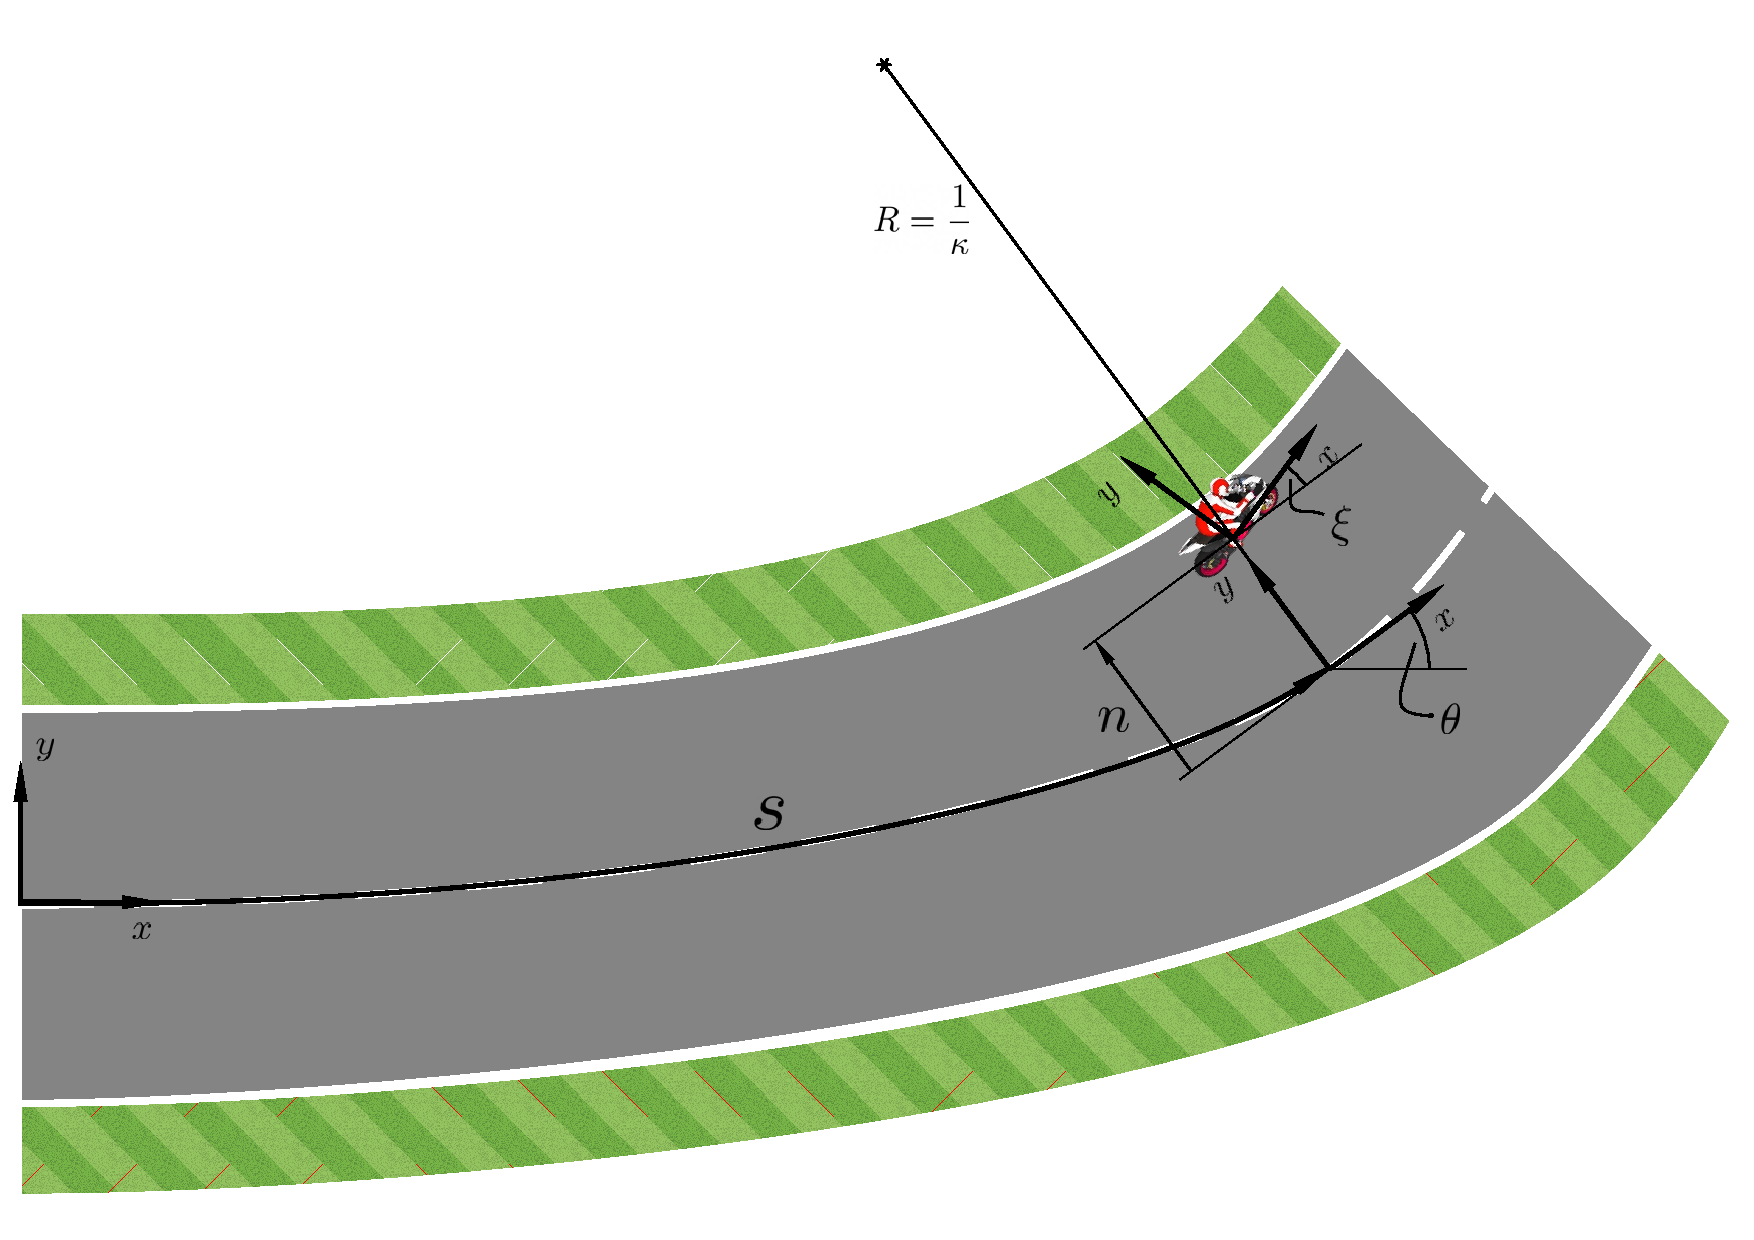
\includegraphics[width=\linewidth]{Coordinates/CurvCoord.pdf}
    \caption{Curvilinear coordinates}
    \label{fig:CurvCoord}
\end{figure}
%
The curvilinear coordinate are a convenient set of coordinate to compute OCPs. This is a well known technique in literature. In this thesis the curvilinear coordinate used consider only a motion on plane (2D). However it can be extended to the three-dimensional space as did by Leonelli and Limebeer \cite{leonelli2019optimal}.\\
%
The curvilinear coordinates ($s(t)$, $n(t)$,$\xi(t)$) can be mapped to quasi states can be obtained defining a reference frame mobile. This is translated with respect to ground of coordinate $\it xm(t)$ and $\it ym(t)$ and rotated around the vertical direction $z$ of an angle $\theta(t)$ (Figure \ref{fig:CurvCoord}).
%
\begin{equation}
\left[ \begin{array}{cccc} 
    \cos \left( \theta \left( t \right) \right) &-\sin \left( \theta \left( t \right)  \right) &0&{\it xm}\left( t \right) \\ 
    \sin \left( \theta \left( t\right)  \right) &\cos \left( \theta \left( t \right)  \right) &0&{\it ym} \left( t \right) \\ 
    0&0&1&0\\ 
    0&0&0&1
\end{array} \right]    
\end{equation}
%
$\theta$ is different from the pitch angle of the previous chapter and will be dropped in the next few passages.\\
From the reference frame previously defined one can define a moving reference frame with longitudinal velocity $\frac {\rm d}{{\rm d}t} s(t)$ and angular velocity $\frac {\rm d}{{\rm d}t} s(t) \kappa(t)$. The last term represent the linear velocity divided by the radius of curvature. In fact $\kappa$ is the curvature of the curvilinear coordinate. $\kappa$ is not a direct function of time. It depends on the curvilinear coordinate $s$, $\kappa(t)=\kappa(s)=\kappa(s(t))$.\\
The velocity of this reference frame are
%
\begin{equation}
    \left[ \begin{array}{c} 
        \displaystyle
        {\frac {\rm d}{{\rm d}t}}s \left( t \right) -\cos \left( \theta \left( t \right)  \right) {\frac {\rm d}{{\rm d}t}}{\it xm} \left( t \right) -\sin \left( \theta \left( t \right) \right) {\frac {\rm d}{{\rm d}t}}{\it ym} \left( t \right) \\
        \displaystyle
        \sin \left( \theta \left( t \right)  \right) {\frac {\rm d}{{\rm d}t}}{\it xm} \left( t \right) -\cos \left( \theta\left( t \right)  \right) {\frac {\rm d}{{\rm d}t}}{\it ym} \left( t\right) \\ 
        \displaystyle
        \kappa \left( t \right) {\frac {\rm d}{{\rm d}t}}s \left( t \right) -{\frac {\rm d}{{\rm d}t}}\theta \left( t\right)
    \end{array} \right]    
\end{equation}
%
From the moving reference frame above mentioned a translation and a rotation are performed. Specifically a lateral translation of $n(t)$ and a rotation of $\xi(t)$. The origin of this reference frame is in fact the position of the motorcycle in the space.
%
\begin{equation}
    \left[ \begin{array}{cccc} 
        \cos \left(\xi \left(t \right)\right)&-\sin \left(\xi \left(t \right)\right)&0&0\\
        \sin \left(\xi \left(t \right)\right)&\cos \left(\xi \left(t \right)\right)&0&n(t)\\
        0&0&1&0\\
        0&0&0&1
    \end{array} \right]  
    \label{eq:refcurv}  
\end{equation}
%
Thus, the velocity of this point can be mapped to the velocity of the vehicle $u(t)$, $v(t)$, $\Omega(t)$. This can be obtained by defining a vector in the reference frame in equation \ref{eq:refcurv} with components $u(t)$ and $v(t)$ and the angular velocity as 
%
\begin{equation}
    \frac{\rm d}{{\rm d}t}\psi(t)-\frac{\rm d}{{\rm d}t}\theta(t)-\frac{\rm d}{{\rm d}t}\xi(t)    
\end{equation}
%
with $\frac{\rm d}{{\rm d}t}\psi(t) = \Omega(t)$ and $\theta(t)=\theta(s(t))$. Moreover the time derivative of $\theta$ can be expressed as 
%
\begin{equation}
    \frac{\rm d}{{\rm d}t}\theta(s(t))=\frac{\rm d}{{\rm d}t}s(t) \frac{\rm d}{{\rm d}s}\theta(s) = \frac{\rm d}{{\rm d}t}s(t) \kappa(s(t))
\end{equation}
%
The terms $\it xm(t)$, $\it ym(t)$ and $\theta(t)$ are no more in the expression and the final equations for the curvilinear coordinates are
%
\begin{equation}
\begin{cases} 
    \displaystyle
    \left( {\frac {\rm d}{{\rm d}t}}s \left( t\right)  \right)  \left( \kappa \left( s \left( t \right)  \right) n\left( t \right) -1 \right) +u \left( t \right) \cos \left( \xi\left( t \right)  \right) -v \left( t \right) \sin \left( \xi \left( t \right)  \right) \\ 
    \displaystyle
    -{\frac {\rm d}{{\rm d}t}}n\left( t \right) +u \left( t \right) \sin \left( \xi \left( t\right)  \right) +v \left( t \right) \cos \left( \xi \left( t\right)  \right) \\ 
    \displaystyle
    \Omega \left( t \right) -\kappa\left( s \left( t \right)  \right) {\frac {\rm d}{{\rm d}t}}s \left( t \right) -{\frac {\rm d}{{\rm d}t}}\xi \left( t \right) 
\end{cases}
\end{equation}
%
Collecting all the differential parts
%
\begin{equation}
    \begin{cases} 
    \displaystyle
    {\frac {\rm d}{{\rm d}t}}s \left( t \right) =-{\frac {u \left( t \right) \cos \left( \xi \left( t \right) \right) -v \left( t \right) \sin \left( \xi \left( t \right) \right) }{\kappa \left( s \left( t \right)  \right) n \left( t\right) -1}}\\
    \displaystyle 
    {\frac {\rm d}{{\rm d}t}}n \left( t\right) =u \left( t \right) \sin \left( \xi \left( t \right) \right) +v \left( t \right) \cos \left( \xi \left( t \right) \right) \\
    \displaystyle
    {\frac {\rm d}{{\rm d}t}}\xi \left( t \right) ={\frac {\kappa \left( s \left( t \right)  \right) u \left( t \right) \cos \left( \xi \left( t \right)  \right) -\kappa \left( s\left( t \right)  \right) v \left( t \right) \sin \left( \xi \left( t\right)  \right) +\kappa \left( s \left( t \right)  \right) n \left( t \right) \Omega \left( t \right) -\Omega \left( t \right) }{\kappa \left( s \left( t \right)  \right) n \left( t \right) -1}}
    \end{cases} 
    \label{eq:CurvCoord}
\end{equation}
%
The last two equation will be integrated in the system of ODE for the OCP while the first will have a central role in the following section.
%